


\section{Experiments}
\label{sec:experiments}
In this section, we explore the techniques via binary classification problems on an artificial dataset (i.e., Moon) and 41 real-world datasets (i.e., KEEL, UCI, Credit Card Fraud). Samples in Moon have two features, while other datasets contain various numbers of features and imbalance ratios. Dataset details are described in Table \ref{tab:dataDecription}.  
The implementation steps to balance datasets follow Algorithm \ref{alg:SIMPOR}. To evaluate our proposed balancing technique, we compare the classification performance to different widely-used and state-of-the-art techniques. More specifically, We compare \Methodname{} to SMOTE \cite{chawla_smote:_2002}, Borderline-SMOTE \cite{bordersmote},  ADASYN \cite{ADASYN}, Random Oversampling (ROS), Gaussian Distribution Based Oversampling (GDO) \cite{bib:GDO}, SVMCS \cite{cssvm}, EE \cite{EE}. To evaluate the classifications performance for skewed datasets, we measure widely-used metrics, i.e., F1-score and Area Under The Curve (AUC).

% Table generated by Excel2LaTeX from sheet 'KEEL Data Description'
\begin{table}[htbp]
	\centering
	\caption{Dataset description.}
	
	\begin{tabular}{lccc}
		\hline
		dataset & \#samples & \#features & IR \\
		\hline
		glass1 & 214   & 9     & 1.8 (138:76)\\
		wisconsin & 683   & 9     & 1.9 (444:239) \\
		pima  & 768   & 8     & 1.9 (500:268)\\
		glass0 & 214   & 9     & 2.1 (144:70) \\
		yeast1 & 1484  & 8     & 2.5 (1055:429)\\
		haberman & 306   & 3     & 2.8 (225:81) \\
		vehicle1 & 846   & 18    & 2.9 (629:217)\\
		vehicle2 & 846   & 18    & 2.9 (628:218)\\
		vehicle3 & 846   & 18    & 3.0 (634:212)\\
		creditcard & 1968  & 30    & 3.0 (1476:492)\\
		glass-0-1-2-3\_vs\_4-5-6 & 214   & 9     & 3.2 (163:51)\\
		vehicle0 & 846   & 18    & 3.3 (647:199)\\
		ecoli1 & 336   & 7     & 3.4 (259:77)\\
		new-thyroid1 & 215   & 5     & 5.1 (180:35) \\
		new-thyroid2 & 215   & 5     & 5.1 (180:35)\\
		ecoli2 & 336   & 7     & 5.5 (284:52)\\
		glass6 & 214   & 9     & 6.4 (185:29)\\
		yeast3 & 1484  & 8     & 8.1 (1321:63)\\
		ecoli3 & 336   & 7     & 8.6 (301:35)\\
		page-blocks0 & 5472  & 10    & 8.8 (4913:559)\\
		yeast-2\_vs\_4 & 514   & 8     & 9.0 (463:51)\\
		yeast-0-5-6-7-9\_vs\_4 & 528   & 8     & 9.4 (477:51)\\
		vowel0 & 988   & 13    & 10.0 (898:90)\\
		glass-0-1-6\_vs\_2 & 192   & 9     & 10.3 (175:17)\\
		glass2 & 214   & 9     & 11.6 (197:17)\\
		yeast-1\_vs\_7 & 459   & 7     & 14.3 (429:30)\\
		glass4 & 214   & 9     & 15.5 (201:13)\\
		ecoli4 & 336   & 7     & 15.8 (316:20)\\
		page-blocks-1-3\_vs\_4 & 472   & 10    & 15.9 (444:28)\\
		abalone9-18 & 731   & 8     & 16.4 (689:42)\\
		yeast-1-4-5-8\_vs\_7 & 693   & 8     & 22.1 (663:30)\\
		glass5 & 214   & 9     & 22.8 (205:9)\\
		yeast-2\_vs\_8 & 482   & 8     & 23.1 (462:20)\\
		car\_eval\_4 & 1728  & 21    & 25.6 (1663:65)\\
		wine\_quality & 4898  & 11    & 25.8 (4715:183)\\
		yeast\_me2 & 1484  & 8     & 28.0 (1433:51)\\
		yeast4 & 1484  & 8     & 28.1 (1433:51)\\
		yeast-1-2-8-9\_vs\_7 & 947   & 8     & 30.6 (917:30)\\
		yeast5 & 1484  & 8     & 32.7 (1440:44)\\
		yeast6 & 1484  & 8     & 41.4 (1449:35)\\
		abalone19 & 4174  & 8     & 129.4 (689:42)\\
	\end{tabular}%
	\label{tab:dataDecription}%
\end{table}%



\subsection{Experimental Setup}
This section describes the general settings and implementation details for the experimental techniques.


\subsubsection{\Methodname{} Settings}
In order to find the informative subset, we leverage entropy-based active learning. We first utilize a neural network model playing a role as a classifier to find high-entropy samples. The detailed steps are introduced in Subsection \ref{sec:EAL}. The model contains two fully connected hidden layers with \textit{relu} activation functions and 100 neurons in each layer. The output layer applies the soft-max activation function. The model is trained in a maximum of 300 epochs with an early stop option until the loss does not change after updating weights. The model is trained firstly on a random set of data; this model is then used to predict the remaining data and compute the sample entropy. We select the top 30 percent of high-entropy samples (IP=0.3) for the informative subsets. Note that the classifier for finding informative subsets differs from the classifiers for the evaluation after all balancing techniques are applied to the data.  

To solve the optimization problem in Equation \ref{prob:optimazation} for finding optima (this differs from the classification optimization for the evaluation) introduced in Section \ref{sec:solvingOptimization}, we use a gradient ascent method with the gradient rate of $1e-5$ and the maximum iteration of 300.   

\subsubsection{Evaluation Classification Settings}
Considering each imbalanced dataset as a classification problem, we use the classification testing performance for the technique comparison. Each dataset is randomly split into two parts, 80\% for training and 20\% for testing. The classifiers are trained on training sets after applying the techniques. The results are reported on the raw testing sets (There isn't any technique applied on the testing sets; thus, they are also possibly class imbalanced). We use F1-score and AUC for the evaluation metrics as they are suitable and widely used to evaluate imbalanced data. Reported testing results for each dataset are the averages of 5 experimental trials.

The classifiers are constructed by neural networks with the input and output sizes corresponding to the number of datasets' features and unique labels. We use the same classifier structure (number of hidden layers, number of neurons in each layer, learning rate, optimizer) for all compared datasets. The detail of neural network implementation is described in Table \ref{tab:model_setting}. 
For baseline technique settings, we follow the experimental parameter sets in \cite{bib:GDO} as we share very similar datasets and comparison techniques.

\begin{table}[htbp]
	\centering
	\caption{Classification model settings for each dataset.}
	%\rule{\linewidth}{3cm}
	\label{tab:model_setting}
	\resizebox{0.7\columnwidth}{!}{%
		
		\begin{tabular}{lp{29.57em}}
			\toprule
			Method & \multicolumn{1}{l}{Parameter} \\
			\midrule
			SIMPOR & \multicolumn{1}{l}{k\_neighbors=5, r\_distribtuion=Gaussian(0,1), IP=0.3} \\
			GDO   & \multicolumn{1}{l}{k\_neighbors=5, d=1} \\
			SMOTE & \multicolumn{1}{l}{k\_neighbors=5, sampling\_strategy=`auto',random\_state=None} \\
			BL-SMOTE & \multicolumn{1}{l}{k\_neighbors=5, sampling\_strategy=`auto', random\_state=None} \\
			ADASYN & \multicolumn{1}{l}{k\_neighbors=5, sampling\_strategy=`auto', random\_state=None} \\
			EE    & \multicolumn{1}{l}{\#estimators=10, Estimater=AdaBoostClassifier} \\
			ROS   & \multicolumn{1}{l}{sampling\_strategy=`auto', random\_state=None, shrinkage=None} \\
			\midrule
			Classifier & \multicolumn{1}{l}{Parameter} \\
			\midrule
			Architecture & \multicolumn{1}{l}{neuron/layer=100, \#layers=3} \\
			Optimization & optimizer=`adam',  epochs=200, batch\_size=32, learning\_rate=0.1, reduce\_lr\_loss(factor=0.9,epsilon=1e-4,patience=5) \\
			\bottomrule
		\end{tabular}%
		
	}
\end{table}%



\subsection{\Methodname{} on Artificial Moon Dataset}


\begin{figure}[htbp!]	
	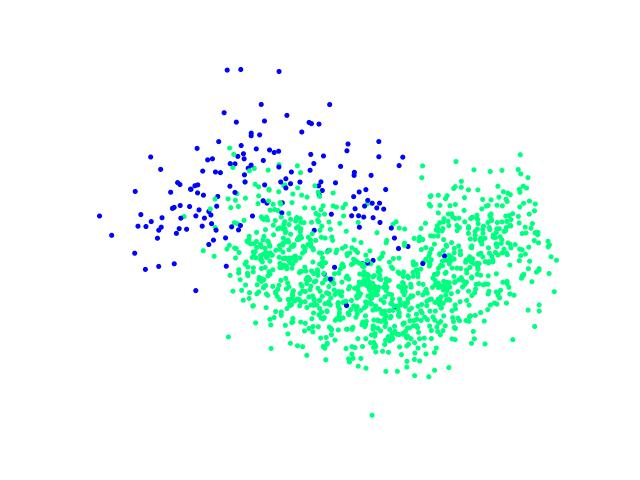
\includegraphics[width=0.9\linewidth]{\ChapterPathSIMPOR/Figures/moon/ImbalancedData}
	\caption{Artificial class imbalanced Moon dataset with IR of 7:1.}
	\label{fig:raw_moon}
\end{figure}


\begin{figure*}[t!]
	\centering
	%[trim=left bottom right top, clip]
	\begin{subfigure}[]{0.3\linewidth}
		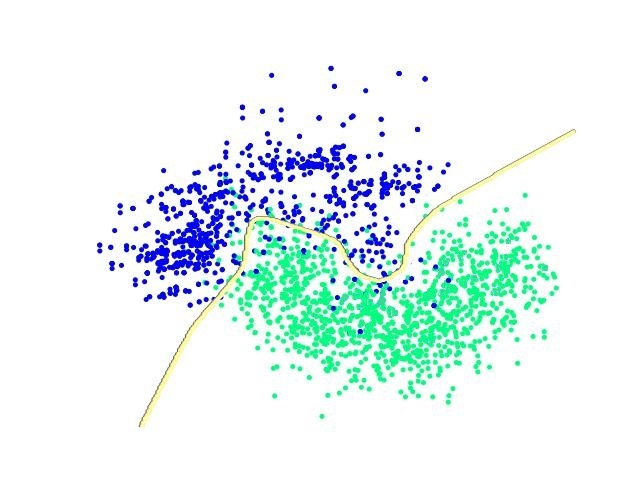
\includegraphics[width=\linewidth]{\ChapterPathSIMPOR/Figures/moon/Training_Data_PLot_SIMPOR}
		\caption{\Methodname{}.}
		\label{fig:simpor_moon}
	\end{subfigure}
	\hspace{0.1em}% 
	\begin{subfigure}[]{0.3\linewidth}
		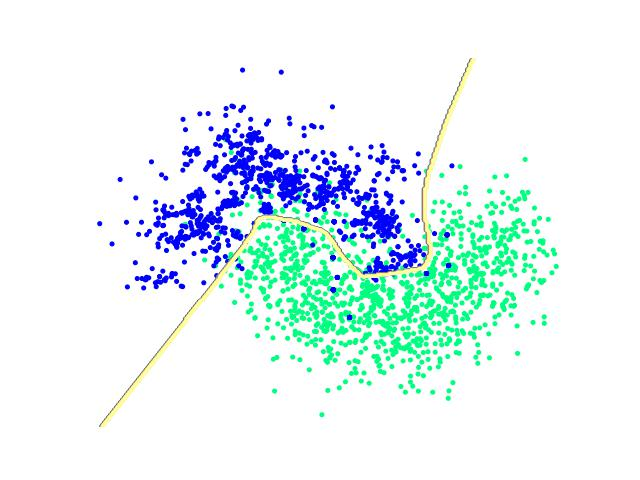
\includegraphics[width=\linewidth]{\ChapterPathSIMPOR/Figures/moon/Training_Data_PLot_GDO}
		\caption{GDO.}
		\label{fig:gdo_moon}
	\end{subfigure}
	\hspace{0.1em}% 
	\begin{subfigure}[]{0.3\linewidth}
		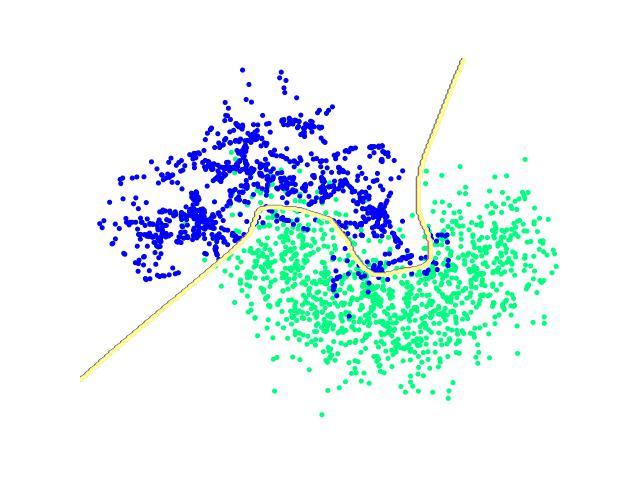
\includegraphics[width=\linewidth]{\ChapterPathSIMPOR/Figures/moon/Training_Data_PLot_SMOTE}
		\caption{SMOTE.}
		\label{fig:smote_moon}
	\end{subfigure}
	\\
	\begin{subfigure}[]{0.3\linewidth}
		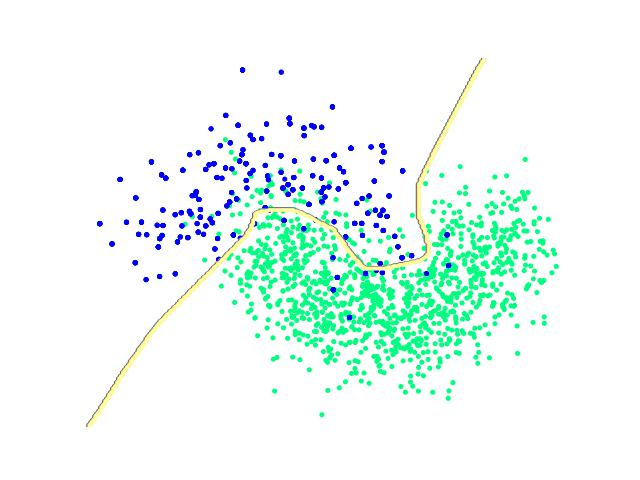
\includegraphics[width=\linewidth]{\ChapterPathSIMPOR/Figures/moon/Training_Data_PLot_ROS}
		\caption{ Random Over Sampling.}
		\label{fig:oversampling_moon}
	\end{subfigure}
	\hspace{0.1em}% 
	\begin{subfigure}[]{0.3\linewidth}
		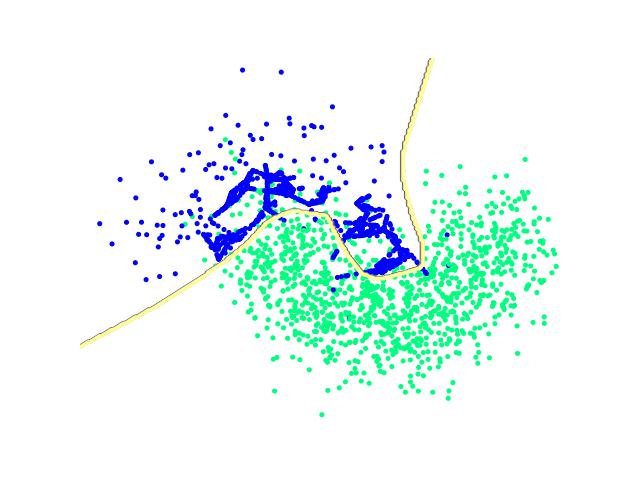
\includegraphics[width=\linewidth]{\ChapterPathSIMPOR/Figures/moon/Training_Data_PLot_BorderlineSMOTE}
		\caption{BorderlineSMOTE.}
		\label{fig:border_smote_moon}
	\end{subfigure}
	\hspace{0.1em}% 
	\begin{subfigure}[]{0.3\linewidth}
		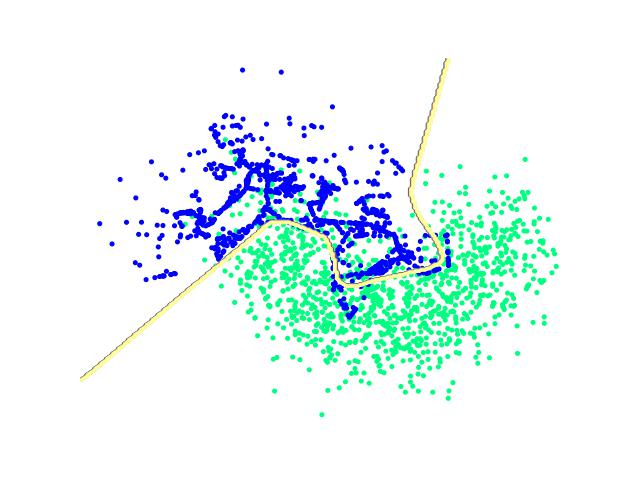
\includegraphics[width=\linewidth]{\ChapterPathSIMPOR/Figures/moon/Training_Data_PLot_ADASYN}
		\caption{ADASYN. }
		\label{fig:adasyn_moon}
	\end{subfigure}
	
	\caption[Data and model decision boundary plot.]{Data plot and model's decision boundary visualization for Moon Dataset over different techniques.}
	\label{fig:MoonResults}
\end{figure*}


We implement techniques on an artificial 2-dimension dataset for demonstration purposes. We first generate the balanced synthetic MOON dataset using \textit{sklearn} package. The generated MOON contains 3000 samples labeled in two classes, and each instance has two numerical features with values ranging from 0 to 1. We then make the dataset artificially imbalanced with an Imbalance Ratio of 7:1 by randomly removing 1285 samples from one class. As a result, the training dataset becomes imbalanced, as visualized in Figure \ref{fig:raw_moon}.

Figure \ref{fig:MoonResults} captures the classification for different techniques. We also visualize the model decision boundaries to provide additional information on how the classification models are affected. We use a fully connected neural network described in Table \ref{tab:model_setting} to classify the data.

% Table generated by Excel2LaTeX from sheet 'Accuracy'
\begin{table}[htbp]
	\centering
	\caption{Classification result on Moon dataset.}
	\resizebox{\columnwidth}{!}{%
		\begin{tabular}{crcccccc}
			Metric &       & SIMPOR & SMOTE & BL-SMOTE & ROS   & ADASYN & GDO \\
			\hline
			F1-score &       & 0.883 & 0.824 & 0.827 & 0.830 & 0.785 & 0.817 \\
			AUC   &       & 0.961 & 0.957 & 0.955 & 0.959 & 0.955 & 0.959 \\
		\end{tabular}%	
	}
	\label{tab:MoonPerformance}
\end{table}%


From the visualization shown in Figure \ref{fig:MoonResults} and the classification performance results in Table \ref{tab:MoonPerformance}, it is clear that \Methodname{} performs better than others by up to 12\% on F1-score and 0.6\% on AUC. We can see that the Random Over Sampling technique (Figure \ref{fig:oversampling_moon}) which randomly duplicates minority samples might push the boundary towards the majority because the samples near the border carry significant weights. Due to the fact that SMOTE does not take the informative region into account, unbalanced data in this area lead to a severe error in decision boundary. In Figures \ref{fig:adasyn_moon} and \ref{fig:border_smote_moon}, BorderlineSMOTE (BL-SMOTE) and ADASYN focus on the area near the model's decision boundary, but they inherit a drawback from SMOTE; any noise or mislabeled samples can, unfortunately, create very dense bridges crossing the expected border and lead to decision errors. Figure \ref{fig:gdo_moon} shows that GDO also generates local gaussian groups of samples near the boder and thus create errors. This phenomenon might cause by a few mis-labeled sample points. In contrast, by generating neighbors of minority samples in the direction towards the minority class and balancing the informative region, \Methodname{} (Figure \ref{fig:simpor_moon}) helps the classifier to make a better decision with a solid smooth decision boundary. Poorly-placed synthetic samples are significantly less than that of others. 


\subsection{\Methodname{} on Forty-one Real Datasets}
\label{subsec:41Datasets}
In this section, we compare the proposed technique on 41 real two-class datasets with a variable number of features and Imbalance Ratios, i.e., KEEL datasets \cite{ KEEL_detail,KEEL_dataset}, UCI datasets fetched from Sklearn tool \cite{imbalancedlearnFetch_datasetsx2014, uci_imbalance_dataset} and Credit Card Fraud \cite{kaggleCreditCard} dataset. Since the original Credit Card Fraud contains a large number of banking normal and fraud transaction samples (284,807) which significantly reduces our experimental efficiency, we reduced the dataset size by randomly removing normal class transactions to reach an imbalance ratio of 3.0. Other datasets are kept as their original versions after removing bad samples (containing Null values). The datasets are described in Table \ref{tab:dataDecription}. 

\subsubsection{Classification Results}
\label{sec:classificationResult}
% Table generated by Excel2LaTeX from sheet 'MacroF1'

\begin{table}[htbp]
	\centering
	\caption{F1-score over different datasets.}
	\resizebox{0.98\columnwidth}{!}{%
		
		\begin{tabular}{lcccccccc}
			\toprule
			& SIMPOR & GDO   & SMOTE & BL-SMOTE & ADASYN & ROS   & SVMCS & EE \\
			\midrule
			glass1 & \textbf{0.746} & 0.694 & 0.709 & 0.720 & 0.702 & 0.699 & 0.724 & 0.705 \\
			wisconsin & 0.967 & \textbf{0.972} & 0.966 & 0.963 & 0.965 & 0.967 & 0.964 & 0.962 \\
			pima  & \textbf{0.754} & 0.733 & 0.716 & 0.728 & 0.737 & 0.731 & 0.740 & 0.749 \\
			glass0 & \textbf{0.817} & 0.786 & 0.798 & 0.794 & 0.776 & 0.778 & 0.801 & \textbf{0.817} \\
			yeast1 & \textbf{0.718} & 0.689 & 0.700 & 0.699 & 0.689 & 0.697 & 0.702 & 0.705 \\
			haberman & 0.591 & 0.614 & 0.617 & 0.611 & \textbf{0.625} & 0.585 & 0.600 & 0.608 \\
			vehicle1 & 0.759 & 0.784 & 0.790 & \textbf{0.791} & 0.789 & 0.773 & 0.754 & 0.768 \\
			vehicle2 & \textbf{0.973} & 0.933 & 0.938 & 0.968 & \textbf{0.973} & 0.958 & 0.971 & 0.970 \\
			vehicle3 & \textbf{0.759} & 0.758 & 0.742 & 0.753 & 0.730 & 0.750 & 0.738 & 0.749 \\
			creditcard & \textbf{0.953} & 0.942 & 0.947 & 0.944 & 0.943 & 0.945 & 0.952 & 0.950 \\
			glass-0-1-2-3\_vs\_4-5-6 & 0.916 & 0.922 & 0.926 & 0.925 & \textbf{0.927} & 0.919 & 0.909 & 0.919 \\
			vehicle0 & 0.960 & 0.948 & 0.954 & 0.962 & 0.968 & 0.967 & \textbf{0.972} & 0.960 \\
			ecoli1 & 0.835 & 0.827 & 0.835 & 0.821 & 0.819 & 0.818 & \textbf{0.849} & 0.838 \\
			new-thyroid1 & 0.957 & 0.956 & 0.957 & 0.957 & \textbf{0.963} & \textbf{0.963} & 0.957 & 0.957 \\
			new-thyroid2 & 0.940 & \textbf{0.978} & 0.934 & 0.940 & 0.940 & 0.940 & 0.934 & 0.934 \\
			ecoli2 & \textbf{0.908} & 0.864 & 0.902 & 0.866 & 0.865 & 0.882 & 0.900 & 0.900 \\
			glass6 & \textbf{0.926} & 0.888 & 0.870 & 0.908 & 0.896 & 0.880 & 0.894 & 0.905 \\
			yeast3 & \textbf{0.878} & 0.833 & 0.856 & 0.846 & 0.843 & 0.854 & 0.870 & 0.877 \\
			ecoli3 & \textbf{0.847} & 0.811 & 0.826 & 0.798 & 0.733 & 0.815 & 0.832 & 0.840 \\
			page-blocks0 & \textbf{0.907} & 0.894 & 0.897 & 0.894 & 0.880 & 0.906 & 0.890 & \textbf{0.907} \\
			yeast-2\_vs\_4 & \textbf{0.881} & 0.842 & 0.868 & 0.859 & 0.861 & 0.878 & 0.795 & 0.786 \\
			yeast-0-5-6-7-9\_vs\_4 & \textbf{0.802} & 0.763 & 0.718 & 0.801 & 0.753 & 0.742 & 0.771 & 0.782 \\
			vowel0 & \textbf{1.000} & \textbf{1.000} & \textbf{1.000} & \textbf{1.000} & \textbf{1.000} & \textbf{1.000} & \textbf{1.000} & \textbf{1.000} \\
			glass-0-1-6\_vs\_2 & 0.661 & 0.707 & 0.686 & 0.694 & \textbf{0.740} & 0.712 & 0.482 & 0.539 \\
			glass2 & 0.638 & 0.710 & 0.775 & 0.757 & \textbf{0.789} & 0.743 & 0.621 & 0.615 \\
			yeast-1\_vs\_7 & \textbf{0.784} & 0.681 & 0.619 & 0.638 & 0.609 & 0.613 & 0.770 & 0.738 \\
			glass4 & \textbf{0.904} & 0.845 & 0.855 & 0.853 & 0.855 & 0.853 & 0.853 & 0.865 \\
			ecoli4 & \textbf{0.900} & 0.857 & 0.872 & 0.880 & 0.865 & 0.872 & 0.888 & 0.888 \\
			page-blocks-1-3\_vs\_4 & 0.974 & 0.948 & 0.965 & 0.971 & 0.977 & 0.959 & \textbf{0.992} & \textbf{0.992} \\
			abalone9-18 & 0.716 & 0.729 & 0.735 & 0.735 & 0.751 & 0.748 & 0.792 & \textbf{0.805} \\
			yeast-1-4-5-8\_vs\_7 & 0.489 & 0.620 & 0.571 & 0.585 & 0.615 & \textbf{0.630} & 0.489 & 0.489 \\
			glass5 & \textbf{0.927} & 0.909 & 0.906 & 0.855 & 0.824 & \textbf{0.927} & 0.665 & 0.664 \\
			yeast-2\_vs\_8 & \textbf{0.832} & 0.703 & 0.712 & 0.708 & 0.691 & 0.747 & \textbf{0.832} & \textbf{0.832} \\
			car\_eval\_4 & \textbf{1.000} & 0.975 & 0.995 & 0.990 & 0.995 & 0.995 & \textbf{1.000} & 0.997 \\
			wine\_quality & \textbf{0.743} & 0.680 & 0.665 & 0.660 & 0.660 & 0.677 & 0.673 & 0.659 \\
			yeast\_me2 & 0.697 & 0.695 & 0.707 & 0.686 & 0.686 & 0.657 & \textbf{0.730} & 0.717 \\
			yeast4 & \textbf{0.743} & 0.693 & 0.650 & 0.682 & 0.668 & 0.677 & 0.731 & 0.740 \\
			yeast-1-2-8-9\_vs\_7 & \textbf{0.762} & 0.637 & 0.604 & 0.615 & 0.618 & 0.608 & 0.738 & 0.731 \\
			yeast5 & 0.843 & 0.844 & 0.889 & 0.888 & \textbf{0.892} & 0.882 & 0.827 & 0.830 \\
			yeast6 & 0.767 & 0.748 & 0.684 & \textbf{0.774} & 0.741 & 0.738 & 0.758 & 0.763 \\
			abalone19 & 0.498 & 0.517 & \textbf{0.541} & 0.524 & 0.537 & 0.533 & 0.498 & 0.498 \\
			\bottomrule
		\end{tabular}%
		
	}
	\label{tab:F1AllDatasets}%
\end{table}%


% Table generated by Excel2LaTeX from sheet 'MicroGmean'
\begin{table}[!htbp]
	\centering
	\caption{AUC result over different datasets.}
	\resizebox{0.98\columnwidth}{!}{%
		
		\begin{tabular}{lcccccccc}
			\toprule
			& SIMPOR & GDO   & SMOTE & BL-SMOTE & ADASYN & ROS   & SVMCS & EE \\
			\midrule
			glass1 & \textbf{0.817} & 0.794 & 0.801 & 0.776 & 0.779 & 0.794 & 0.795 & 0.783 \\
			wisconsin & \textbf{0.996} & 0.995 & 0.995 & 0.993 & 0.994 & 0.995 & 0.995 & \textbf{0.996} \\
			pima  & \textbf{0.849} & 0.825 & 0.818 & 0.811 & 0.816 & 0.820 & 0.832 & 0.834 \\
			glass0 & \textbf{0.897} & 0.878 & 0.877 & 0.870 & 0.866 & 0.873 & 0.882 & 0.882 \\
			yeast1 & \textbf{0.810} & 0.777 & 0.785 & 0.784 & 0.770 & 0.785 & 0.799 & 0.801 \\
			haberman & \textbf{0.724} & 0.680 & 0.680 & 0.669 & 0.678 & 0.676 & 0.699 & 0.693 \\
			vehicle1 & 0.901 & 0.903 & 0.907 & 0.901 & 0.895 & 0.893 & \textbf{0.911} & 0.909 \\
			vehicle2 & \textbf{0.998} & 0.994 & 0.972 & 0.994 & 0.997 & \textbf{0.998} & 0.997 & 0.996 \\
			vehicle3 & \textbf{0.892} & 0.869 & 0.880 & 0.876 & 0.841 & 0.877 & 0.879 & 0.876 \\
			creditcard & \textbf{0.974} & 0.973 & 0.967 & 0.963 & 0.969 & 0.966 & 0.971 & 0.972 \\
			glass-0-1-2-3\_vs\_4-5-6 & \textbf{0.992} & 0.990 & 0.985 & 0.986 & 0.976 & 0.990 & 0.988 & 0.988 \\
			vehicle0 & 0.994 & 0.993 & 0.993 & 0.994 & 0.993 & 0.994 & \textbf{0.995} & 0.994 \\
			ecoli1 & \textbf{0.956} & 0.949 & 0.954 & 0.945 & 0.948 & 0.940 & 0.954 & 0.953 \\
			new-thyroid1 & 0.997 & \textbf{0.999} & 0.998 & 0.998 & 0.997 & 0.997 & 0.998 & 0.998 \\
			new-thyroid2 & 0.998 & \textbf{0.999} & 0.998 & 0.998 & 0.998 & 0.998 & \textbf{0.999} & \textbf{0.999} \\
			ecoli2 & \textbf{0.959} & 0.951 & 0.955 & 0.936 & 0.948 & 0.955 & 0.949 & 0.953 \\
			glass6 & 0.905 & \textbf{0.956} & 0.925 & 0.876 & 0.890 & 0.936 & 0.926 & 0.946 \\
			yeast3 & \textbf{0.974} & 0.960 & 0.963 & 0.956 & 0.954 & 0.953 & \textbf{0.974} & \textbf{0.974} \\
			ecoli3 & \textbf{0.902} & 0.892 & 0.886 & 0.883 & 0.833 & 0.889 & 0.885 & 0.895 \\
			page-blocks0 & 0.986 & \textbf{0.988} & 0.983 & 0.984 & 0.985 & 0.987 & 0.983 & 0.983 \\
			yeast-2\_vs\_4 & \textbf{0.982} & 0.975 & 0.958 & 0.969 & 0.948 & 0.961 & 0.949 & 0.930 \\
			yeast-0-5-6-7-9\_vs\_4 & \textbf{0.918} & 0.914 & 0.864 & 0.908 & 0.879 & 0.815 & 0.891 & 0.892 \\
			vowel0 & \textbf{1.000} & \textbf{1.000} & \textbf{1.000} & \textbf{1.000} & \textbf{1.000} & \textbf{1.000} & \textbf{1.000} & \textbf{1.000} \\
			glass-0-1-6\_vs\_2 & 0.868 & 0.849 & 0.892 & 0.871 & 0.893 & \textbf{0.895} & 0.870 & 0.885 \\
			glass2 & 0.903 & 0.903 & 0.918 & 0.906 & \textbf{0.924} & 0.903 & 0.900 & 0.897 \\
			yeast-1\_vs\_7 & \textbf{0.870} & 0.816 & 0.738 & 0.783 & 0.742 & 0.755 & 0.825 & 0.817 \\
			glass4 & \textbf{0.992} & 0.975 & 0.977 & 0.979 & 0.969 & 0.957 & 0.985 & 0.982 \\
			ecoli4 & \textbf{0.988} & 0.979 & 0.985 & 0.981 & 0.981 & 0.946 & 0.986 & 0.986 \\
			page-blocks-1-3\_vs\_4 & 0.998 & \textbf{0.999} & \textbf{0.999} & \textbf{0.999} & \textbf{0.999} & 0.998 & \textbf{0.999} & \textbf{0.999} \\
			abalone9-18 & 0.898 & 0.925 & \textbf{0.935} & 0.919 & 0.932 & 0.921 & 0.916 & 0.921 \\
			yeast-1-4-5-8\_vs\_7 & \textbf{0.801} & 0.770 & 0.692 & 0.705 & 0.704 & 0.741 & 0.746 & 0.747 \\
			glass5 & \textbf{1.000} & 0.996 & 0.995 & 0.988 & 0.990 & 0.951 & 0.995 & 0.995 \\
			yeast-2\_vs\_8 & \textbf{0.823} & 0.737 & 0.783 & 0.789 & 0.772 & 0.763 & 0.797 & 0.787 \\
			car\_eval\_4 & \textbf{1.000} & \textbf{1.000} & \textbf{1.000} & \textbf{1.000} & \textbf{1.000} & \textbf{1.000} & \textbf{1.000} & \textbf{1.000} \\
			wine\_quality & \textbf{0.859} & 0.802 & 0.752 & 0.787 & 0.756 & 0.782 & 0.826 & 0.825 \\
			yeast\_me2 & \textbf{0.920} & 0.903 & 0.875 & 0.864 & 0.848 & 0.871 & 0.896 & 0.905 \\
			yeast4 & \textbf{0.907} & 0.893 & 0.805 & 0.836 & 0.821 & 0.809 & 0.854 & 0.858 \\
			yeast-1-2-8-9\_vs\_7 & \textbf{0.823} & 0.767 & 0.709 & 0.729 & 0.710 & 0.752 & 0.784 & 0.770 \\
			yeast5 & \textbf{0.993} & 0.991 & \textbf{0.993} & 0.992 & \textbf{0.993} & \textbf{0.993} & 0.992 & \textbf{0.993} \\
			yeast6 & \textbf{0.968} & 0.940 & 0.851 & 0.944 & 0.935 & 0.936 & 0.956 & 0.952 \\
			abalone19 & \textbf{0.806} & 0.640 & 0.672 & 0.675 & 0.683 & 0.669 & 0.780 & 0.784 \\
			\bottomrule
		\end{tabular}%
		
	}
	\label{tab:AUCAllDatasets}%
\end{table}%


\begin{table}[!htbp]
	\centering
	\caption{Precision results over 41 datasets.}
	\resizebox{0.98\columnwidth}{!}{%
		
		\begin{tabular}{lcccccccc}
			\toprule
			& SIMPOR & GDO   & SMOTE & BL-SMOTE & ADASYN & ROS   & SVMCS & EE \\
			\midrule
			glass1 & \textbf{0.755} & 0.695 & 0.714 & 0.720 & 0.701 & 0.699 & 0.729 & 0.714 \\
			wisconsin & \textbf{0.965} & \textbf{0.965} & 0.962 & 0.959 & 0.961 & 0.964 & 0.963 & 0.960 \\
			pima  & \textbf{0.762} & 0.727 & 0.713 & 0.722 & 0.731 & 0.727 & 0.747 & 0.755 \\
			glass0 & \textbf{0.816} & 0.774 & 0.790 & 0.780 & 0.764 & 0.766 & 0.796 & 0.813 \\
			yeast1 & \textbf{0.734} & 0.676 & 0.688 & 0.685 & 0.676 & 0.688 & 0.722 & 0.725 \\
			haberman & 0.628 & 0.607 & 0.614 & 0.600 & 0.614 & 0.581 & 0.643 & \textbf{0.646} \\
			vehicle1 & 0.760 & 0.767 & 0.778 & \textbf{0.785} & 0.774 & 0.756 & 0.774 & 0.784 \\
			vehicle2 & 0.967 & 0.916 & 0.955 & 0.969 & 0.968 & 0.948 & \textbf{0.970} & 0.964 \\
			vehicle3 & \textbf{0.768} & 0.733 & 0.736 & 0.739 & 0.719 & 0.738 & 0.745 & 0.751 \\
			creditcard & 0.959 & 0.945 & 0.952 & 0.950 & 0.951 & 0.956 & \textbf{0.971} & 0.964 \\
			glass-0-1-2-3\_vs\_4-5-6 & 0.911 & 0.894 & \textbf{0.924} & \textbf{0.924} & 0.921 & 0.913 & 0.909 & 0.920 \\
			vehicle0 & \textbf{0.966} & 0.926 & 0.951 & 0.952 & 0.965 & 0.955 & 0.965 & 0.962 \\
			ecoli1 & 0.845 & 0.819 & 0.815 & 0.795 & 0.799 & 0.803 & \textbf{0.848} & 0.840 \\
			new-thyroid1 & 0.960 & 0.940 & 0.960 & 0.960 & \textbf{0.963} & \textbf{0.963} & 0.960 & 0.960 \\
			new-thyroid2 & 0.963 & \textbf{0.976} & 0.961 & 0.963 & 0.963 & 0.963 & 0.961 & 0.961 \\
			ecoli2 & \textbf{0.924} & 0.839 & 0.903 & 0.851 & 0.851 & 0.867 & 0.915 & 0.915 \\
			glass6 & 0.976 & 0.926 & 0.929 & \textbf{0.984} & 0.959 & 0.949 & 0.982 & \textbf{0.984} \\
			yeast3 & \textbf{0.885} & 0.778 & 0.819 & 0.814 & 0.821 & 0.815 & 0.871 & 0.883 \\
			ecoli3 & 0.856 & 0.748 & 0.773 & 0.739 & 0.679 & 0.763 & 0.847 & \textbf{0.859} \\
			page-blocks0 & 0.927 & 0.846 & 0.865 & 0.844 & 0.824 & 0.865 & \textbf{0.929} & 0.921 \\
			yeast-2\_vs\_4 & \textbf{0.897} & 0.821 & 0.873 & 0.864 & 0.865 & 0.894 & 0.739 & 0.803 \\
			yeast-0-5-6-7-9\_vs\_4 & \textbf{0.839} & 0.715 & 0.731 & 0.775 & 0.767 & 0.726 & 0.822 & 0.833 \\
			vowel0 & \textbf{1.000} & \textbf{1.000} & \textbf{1.000} & \textbf{1.000} & \textbf{1.000} & \textbf{1.000} & \textbf{1.000} & \textbf{1.000} \\
			glass-0-1-6\_vs\_2 & 0.713 & 0.636 & 0.661 & 0.671 & 0.730 & \textbf{0.750} & 0.465 & 0.535 \\
			glass2 & 0.692 & 0.643 & 0.718 & 0.701 & \textbf{0.724} & 0.696 & 0.642 & 0.625 \\
			yeast-1\_vs\_7 & \textbf{0.944} & 0.631 & 0.589 & 0.623 & 0.577 & 0.601 & 0.932 & 0.904 \\
			glass4 & \textbf{0.945} & 0.784 & 0.875 & 0.898 & 0.875 & 0.898 & 0.942 & 0.918 \\
			ecoli4 & \textbf{0.902} & 0.795 & 0.848 & 0.862 & 0.838 & 0.848 & 0.877 & 0.877 \\
			page-blocks-1-3\_vs\_4 & \textbf{0.997} & 0.908 & 0.937 & 0.948 & 0.959 & 0.927 & 0.986 & 0.986 \\
			abalone9-18 & 0.837 & 0.658 & 0.650 & 0.672 & 0.685 & 0.676 & \textbf{0.942} & 0.933 \\
			yeast-1-4-5-8\_vs\_7 & 0.479 & 0.571 & 0.548 & 0.561 & 0.566 & \textbf{0.581} & 0.479 & 0.479 \\
			glass5 & \textbf{0.995} & 0.852 & 0.961 & 0.869 & 0.842 & 0.971 & 0.687 & 0.687 \\
			yeast-2\_vs\_8 & \textbf{0.883} & 0.674 & 0.656 & 0.688 & 0.629 & 0.736 & \textbf{0.883} & \textbf{0.883} \\
			car\_eval\_4 & \textbf{1.000} & 0.954 & 0.990 & 0.981 & 0.990 & 0.990 & \textbf{1.000} & \textbf{1.000} \\
			wine\_quality & \textbf{0.809} & 0.658 & 0.673 & 0.650 & 0.674 & 0.684 & 0.767 & 0.719 \\
			yeast\_me2 & 0.788 & 0.609 & 0.662 & 0.661 & 0.657 & 0.620 & \textbf{0.922} & 0.887 \\
			yeast4 & 0.859 & 0.614 & 0.604 & 0.637 & 0.613 & 0.632 & 0.815 & \textbf{0.888} \\
			yeast-1-2-8-9\_vs\_7 & \textbf{0.989} & 0.580 & 0.564 & 0.602 & 0.577 & 0.592 & 0.988 & 0.988 \\
			yeast5 & 0.835 & 0.748 & 0.833 & 0.840 & 0.835 & 0.816 & \textbf{0.859} & 0.836 \\
			yeast6 & 0.827 & 0.645 & 0.616 & 0.740 & 0.658 & 0.691 & \textbf{0.831} & 0.810 \\
			abalone19 & 0.497 & 0.510 & 0.513 & 0.506 & 0.506 & \textbf{0.517} & 0.497 & 0.497 \\
			\bottomrule
		\end{tabular}%
		
	}
	\label{tab:Precision}%
\end{table}%

\begin{table}[!htbp]
	\centering
	\caption{Recall results over 41 datasets.}
	\resizebox{0.98\columnwidth}{!}{%
		
		\begin{tabular}{lcccccccc}
			\toprule
			& SIMPOR & GDO   & SMOTE & BL-SMOTE & ADASYN & ROS   & SVMCS & EE \\
			\midrule
			glass1 & \textbf{0.738} & 0.693 & 0.705 & 0.719 & 0.702 & 0.698 & 0.718 & 0.697 \\
			wisconsin & 0.969 & \textbf{0.978} & 0.969 & 0.967 & 0.969 & 0.970 & 0.966 & 0.964 \\
			pima  & \textbf{0.746} & 0.740 & 0.720 & 0.734 & 0.744 & 0.735 & 0.734 & 0.742 \\
			glass0 & 0.818 & 0.799 & 0.807 & 0.809 & 0.789 & 0.792 & 0.807 & \textbf{0.821} \\
			yeast1 & 0.702 & 0.702 & \textbf{0.713} & \textbf{0.713} & 0.702 & 0.706 & 0.683 & 0.685 \\
			haberman & 0.559 & 0.622 & 0.621 & 0.623 & \textbf{0.638} & 0.590 & 0.565 & 0.578 \\
			vehicle1 & 0.759 & 0.802 & 0.803 & 0.798 & \textbf{0.806} & 0.792 & 0.738 & 0.755 \\
			vehicle2 & 0.978 & 0.951 & 0.926 & 0.967 & \textbf{0.979} & 0.968 & 0.972 & 0.975 \\
			vehicle3 & 0.751 & \textbf{0.785} & 0.749 & 0.768 & 0.742 & 0.762 & 0.732 & 0.750 \\
			creditcard & \textbf{0.947} & 0.940 & 0.942 & 0.938 & 0.936 & 0.935 & 0.933 & 0.936 \\
			glass-0-1-2-3\_vs\_4-5-6 & 0.924 & \textbf{0.951} & 0.929 & 0.927 & 0.935 & 0.925 & 0.909 & 0.919 \\
			vehicle0 & 0.954 & 0.972 & 0.957 & 0.973 & 0.970 & \textbf{0.980} & 0.979 & 0.959 \\
			ecoli1 & 0.828 & 0.837 & \textbf{0.857} & 0.849 & 0.841 & 0.837 & 0.851 & 0.838 \\
			new-thyroid1 & 0.953 & \textbf{0.972} & 0.953 & 0.953 & 0.963 & 0.963 & 0.953 & 0.953 \\
			new-thyroid2 & 0.920 & \textbf{0.981} & 0.910 & 0.920 & 0.920 & 0.920 & 0.910 & 0.910 \\
			ecoli2 & 0.893 & 0.891 & \textbf{0.902} & 0.883 & 0.882 & 0.897 & 0.885 & 0.885 \\
			glass6 & \textbf{0.888} & 0.854 & 0.819 & 0.843 & 0.841 & 0.821 & 0.823 & 0.840 \\
			yeast3 & 0.871 & \textbf{0.897} & 0.895 & 0.881 & 0.869 & 0.896 & 0.869 & 0.871 \\
			ecoli3 & 0.841 & \textbf{0.886} & \textbf{0.886} & 0.867 & 0.797 & 0.875 & 0.822 & 0.824 \\
			page-blocks0 & 0.888 & 0.948 & 0.932 & 0.951 & 0.945 & \textbf{0.952} & 0.856 & 0.894 \\
			yeast-2\_vs\_4 & 0.867 & \textbf{0.868} & 0.865 & 0.856 & 0.858 & 0.865 & \textbf{0.868} & 0.805 \\
			yeast-0-5-6-7-9\_vs\_4 & 0.770 & 0.827 & 0.706 & \textbf{0.832} & 0.763 & 0.759 & 0.728 & 0.740 \\
			vowel0 & \textbf{1.000} & \textbf{1.000} & \textbf{1.000} & \textbf{1.000} & \textbf{1.000} & \textbf{1.000} & \textbf{1.000} & \textbf{1.000} \\
			glass-0-1-6\_vs\_2 & 0.625 & \textbf{0.807} & 0.725 & 0.727 & 0.760 & 0.709 & 0.500 & 0.545 \\
			glass2 & 0.602 & 0.797 & 0.853 & 0.833 & \textbf{0.875} & 0.803 & 0.607 & 0.607 \\
			yeast-1\_vs\_7 & 0.678 & \textbf{0.744} & 0.654 & 0.656 & 0.647 & 0.626 & 0.662 & 0.628 \\
			glass4 & 0.873 & \textbf{0.921} & 0.848 & 0.830 & 0.848 & 0.830 & 0.786 & 0.832 \\
			ecoli4 & 0.904 & \textbf{0.936} & 0.900 & 0.901 & 0.899 & 0.900 & 0.902 & 0.902 \\
			page-blocks-1-3\_vs\_4 & 0.952 & 0.993 & 0.996 & 0.996 & 0.997 & 0.995 & \textbf{0.999} & \textbf{0.999} \\
			abalone9-18 & 0.631 & 0.819 & \textbf{0.846} & 0.814 & 0.835 & 0.842 & 0.693 & 0.716 \\
			yeast-1-4-5-8\_vs\_7 & 0.500 & 0.689 & 0.600 & 0.615 & 0.688 & \textbf{0.697} & 0.500 & 0.500 \\
			glass5 & 0.875 & \textbf{0.988} & 0.865 & 0.848 & 0.813 & 0.898 & 0.650 & 0.648 \\
			yeast-2\_vs\_8 & 0.797 & 0.778 & \textbf{0.802} & 0.767 & 0.783 & 0.790 & 0.797 & 0.797 \\
			car\_eval\_4 & \textbf{1.000} & 0.998 & \textbf{1.000} & 0.999 & \textbf{1.000} & \textbf{1.000} & \textbf{1.000} & 0.994 \\
			wine\_quality & 0.689 & \textbf{0.704} & 0.657 & 0.672 & 0.647 & 0.672 & 0.602 & 0.608 \\
			yeast\_me2 & 0.627 & \textbf{0.811} & 0.763 & 0.714 & 0.719 & 0.706 & 0.610 & 0.609 \\
			yeast4 & 0.663 & \textbf{0.795} & 0.705 & 0.735 & 0.734 & 0.732 & 0.667 & 0.643 \\
			yeast-1-2-8-9\_vs\_7 & 0.620 & \textbf{0.710} & 0.652 & 0.629 & 0.667 & 0.630 & 0.589 & 0.580 \\
			yeast5 & 0.862 & \textbf{0.972} & 0.959 & 0.951 & 0.963 & 0.965 & 0.819 & 0.836 \\
			yeast6 & 0.735 & \textbf{0.894} & 0.777 & 0.812 & 0.854 & 0.805 & 0.706 & 0.730 \\
			abalone19 & 0.500 & 0.525 & 0.574 & 0.546 & \textbf{0.581} & 0.552 & 0.500 & 0.500 \\
			\bottomrule
		\end{tabular}%
		
	}
	\label{tab:Recall}%
\end{table}%


\begin{figure}[h!]
	\centering
	%[trim=left bottom right top, clip]
	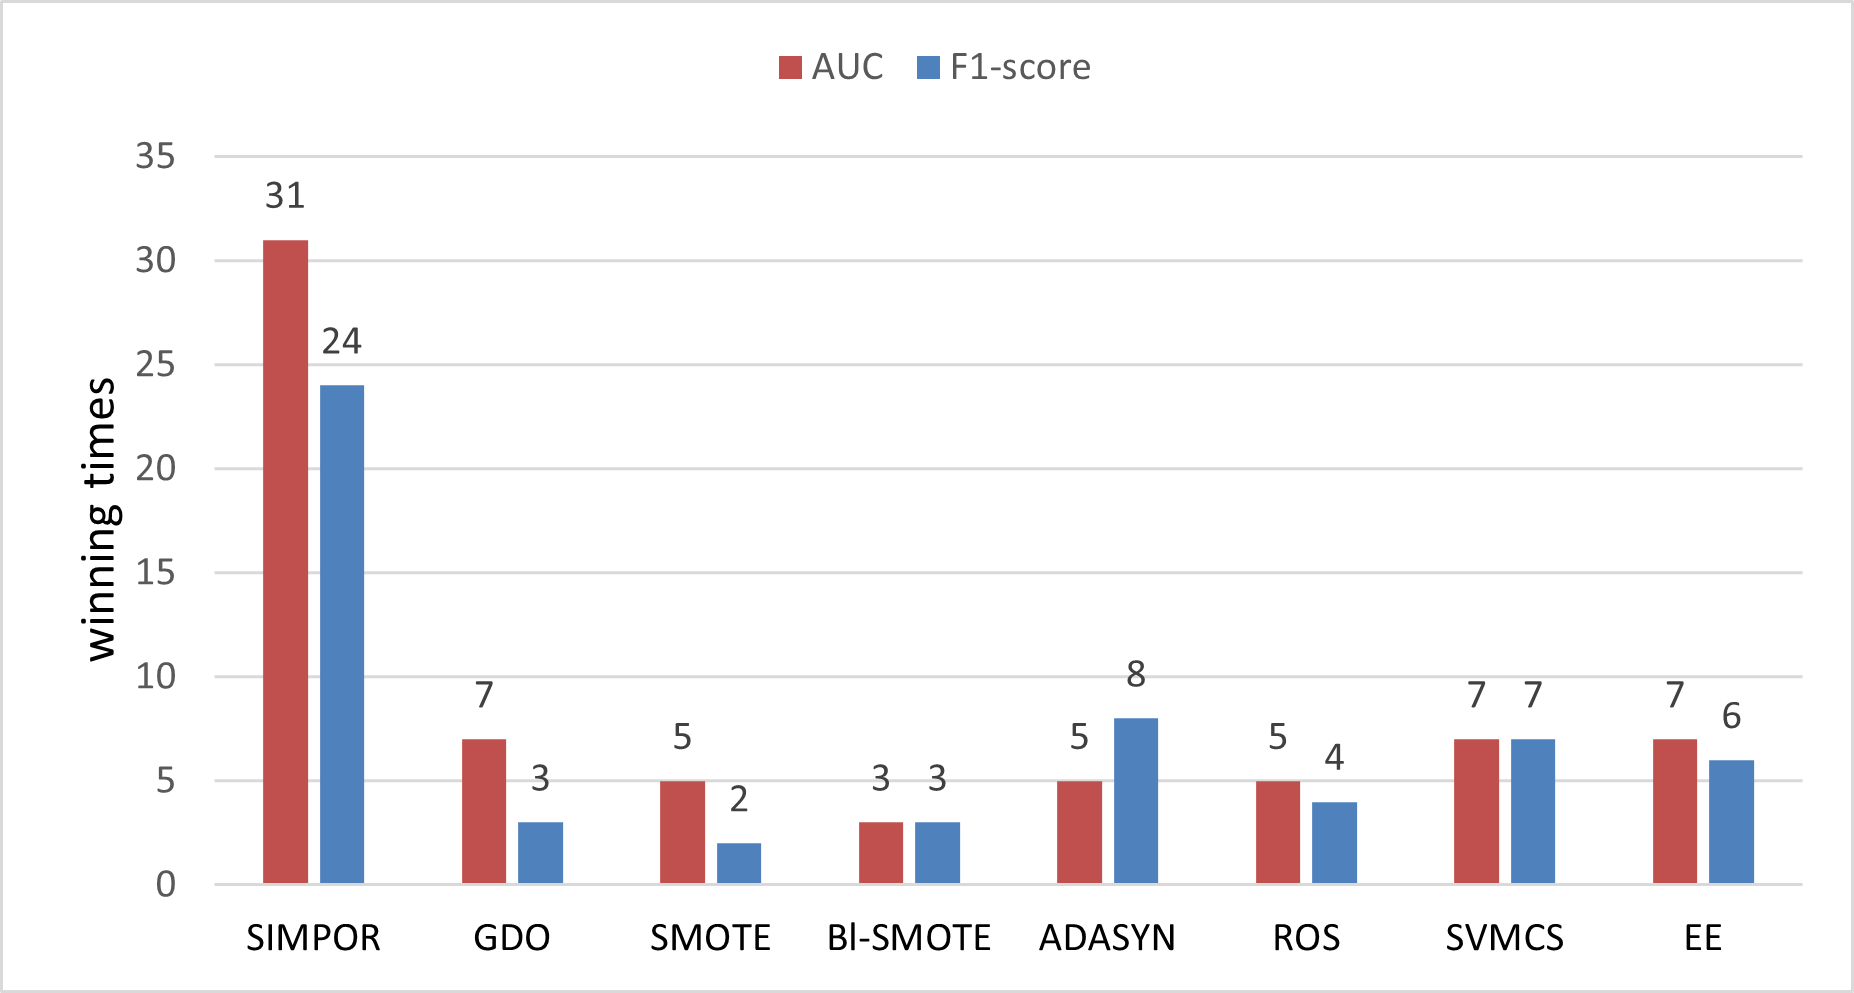
\includegraphics[width=\linewidth ]{\ChapterPathSIMPOR/Figures/winning_times}
	\caption{Winning times over 41 datasets.}
	\label{fig:winingTimes}
\end{figure}

Table \ref{tab:F1AllDatasets}, \ref{tab:AUCAllDatasets}, \ref{tab:Precision} and \ref{tab:Recall} show the classification F1-score, AUC, Precision, and Recall results, respectively. The highest scores for each dataset are highlighted in bold style. 
We also provide the summary of the F1 and AUC scores by ``winning times" scores. We count the number of datasets for which a technique achieves the highest scores among the compared techniques and name this number ``winning times". For convention, if more than two techniques share the same highest score, the winning times will be increased for each technique. Figure \ref{fig:winingTimes} shows a summary of winning times.

As we can see from the table, the proposed technique outperforms others on both evaluation metrics, F1-score and AUC. More specifically, \Methodname{} hits 24 F1-score winning times and 31 AUC winning times. Its number of F1-score winning times at 24 tripled the second winner (ADASYN) at 8, and its AUC winning times at 31 is far from the second AUC winners (GDO, EE, SVMCS) at 7. 


\subsubsection{Statistical Test}
\label{sec:wilcoxon}

To further evaluate the effectiveness of the technique, we also performed a Wilcoxon Signed Rank Test \cite{wilcoxon} on the 41 dataset results (F1 score and AUC). Wilcoxon hypothesis test is relevant to our study as it is a non-parametric statistical test and does not require a specific distribution assumption for the results. On the other hand, 41 data points (corresponding to 41 datasets results) are sufficient to support this test. Our null hypothesis is that the difference between the proposed technique results and those of the other technique is insignificant. Wilcoxon signed-rank test outputs are computed over the 41 dataset results and return a p-value for each technique pair. We then compare the p-value with the significant value $\alpha = 0.05$. Suppose the p-value is smaller than $\alpha$. In that case, the evidence is sufficient to reject the hypothesis, which means the proposed technique does make a significant difference from the others, and vice versa. Table \ref{tab:wilcoxonTest} shows the Wilcoxon p-value results.

\begin{table}[htbp]
	\centering
	\caption{Wilcoxon signed rank hypothesis test results.}
	
	\begin{tabular}{lcc}
		\toprule
		& \multicolumn{2}{c}{p-value} \\
		\midrule
		SIMPOR vs. & \multicolumn{1}{l|}{F1-score} & \multicolumn{1}{l}{AUC} \\
		\midrule
		GDO   & 4.96E-03 & 4.99E-05 \\
		SMOTE & 2.32E-02 & 1.27E-04 \\
		BL\_SMOTE & 2.90E-02 & 3.06E-06 \\
		ADASYN & 3.30E-02 & 1.35E-05 \\
		ROS   & 1.39E-02 & 5.58E-05 \\
		SVMCS & 1.44E-03 & 5.80E-05 \\
		EE    & 2.82E-03 & 3.33E-04 \\
		\bottomrule
	\end{tabular}%
	
	
	\label{tab:wilcoxonTest}%
\end{table}%


As we can see from Table \ref{tab:wilcoxonTest}, the p-values are all smaller than the critical value of 0.05. Thus, the null hypothesis can be rejected as the supporting evidence is sufficient. In other words, the statistical result shows that the proposed technique makes a significant improvement compared to others.     




\subsubsection{Data Visualization}  

\begin{figure*}[h!]
	\centering
	%[trim=left bottom right top, clip]
	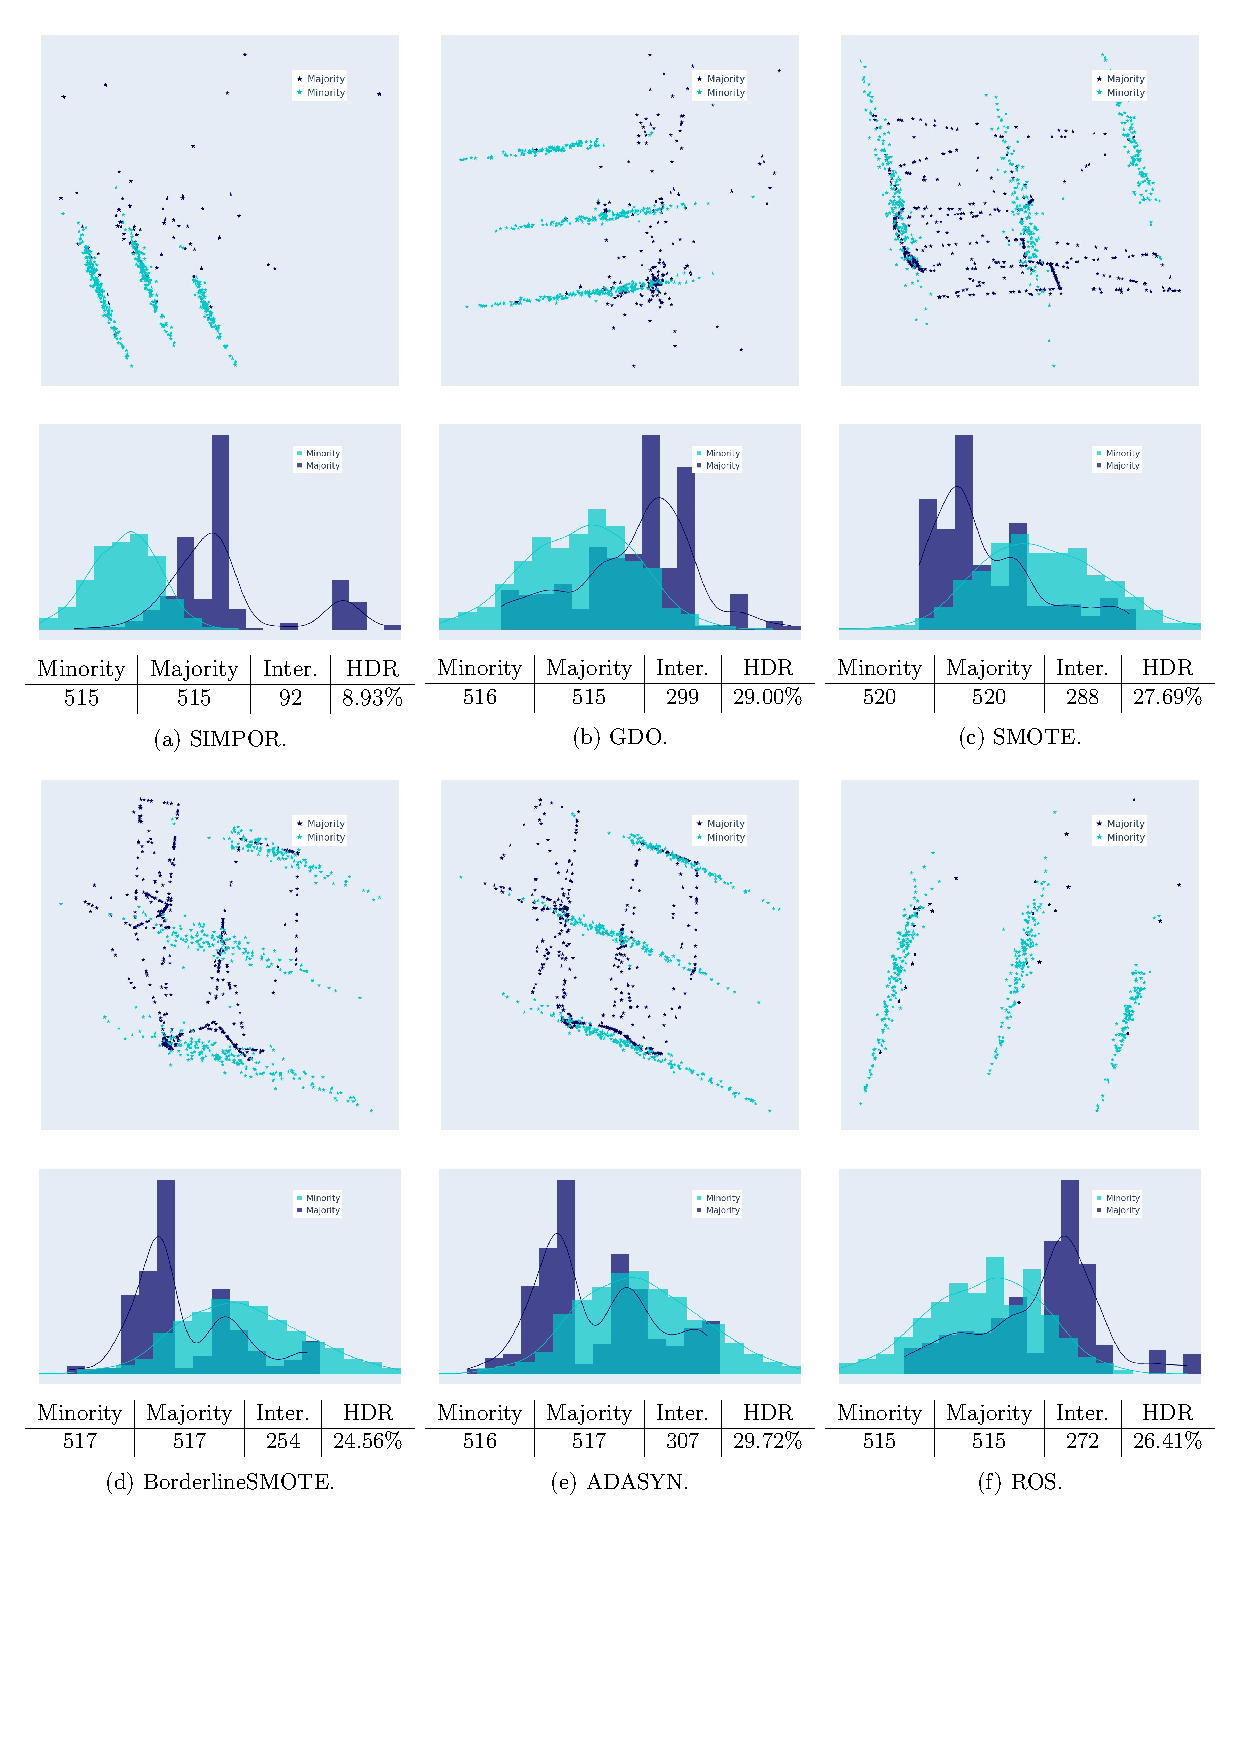
\includegraphics[width=0.8\linewidth,trim=10 90 10 10, clip ]{\ChapterPathSIMPOR/Figures/PCA/abalone9-18}
	\caption[Data visualization over methods.]{Abalone9-18: Generated training data projected onto 2-dimension space and their histograms in 1-Dimension space using Principle Component Analysis dimension reduction technique. The bottom tables illustrate the number of samples in two classes, 1-Dimension histogram intersection between 2 classes, and the hard-to-differentiate ratio between the number of intersectional samples to the number of minority samples ($HDR = \frac{Inter.}{Minority}100\%$).}
	\label{fig:visualization1d2d}
\end{figure*}

To explore more on how the techniques perform, we visualize the generated data by projecting them onto lower dimension space (i.e., one and two dimensions) using the Principle Component Analysis technique (PCA) \cite{PCA}. Data's 2-Dimension (2D) plots and 1-Dimension histograms are presented along with a hard-to-differentiate ratio (HDR) for each technique. A hard-to-differentiate ratio is defined as the ratio of intersection between 2 classes in the 1D histogram to the total of minority samples ($HDR = \frac{No.\: Intersection \: samples}{No. \: Minority \: samples} $). This ratio is expected to be as small as 0\% if the two classes are well separated; in contrast, 100\% indicates that the two classes are unable to be distinguished in the projected 1D space. Other than HDR, we show the absolute numbers of Minority, Majority, and Intersection samples for each technique in the bottom tables. From the plots, we observe how the data are distributed in 2D space and quantify samples that are hard to be differentiated in the 1D space histograms.    

To save space, we only show the plot of one dataset (i.e., Abalone9-18 dataset) in Figure \ref{fig:visualization1d2d}. Many other datasets are observed to have similar patterns. We observe that the proposed technique does not poorly generate synthetic samples as many as other techniques do. HDR results show that \Methodname{} achieves the least number of hard-to-differentiate ratio at 8.93\%. As shown in the 2D visualization sub-figures, other techniques poorly-place synthetic data crossed the other class. This causes by outliers or noises near the border between the two classes that other techniques do not pay attention to and mistakenly create more noise. In contrast, \Methodname{} safely produces synthetic data towards the minority class by maximizing the posterior ratio ;thus it can reduce the number of poorly-places samples.

\begin{table}[htbp]
	\centering
	\caption[Processing time]{Processing time (in seconds) over 41 datasets.}
	\resizebox{0.98\columnwidth}{!}{%
		
		\begin{tabular}{lcccccc}
			\toprule
			& SIMPOR & GDO   & SMOTE & BL-SMOTE & ADASYN & ROS \\
			\midrule
			glass1 & 0.1147 & 0.0576 & 0.0020 & 0.0033 & 0.0032 & 0.0007 \\
			wisconsin & 2.0805 & 0.1769 & 0.0024 & 0.0044 & 0.0046 & 0.0007 \\
			pima  & 0.2032 & 0.2066 & 0.0025 & 0.0049 & 0.0050 & 0.0006 \\
			glass0 & 0.2157 & 0.0553 & 0.0023 & 0.0035 & 0.0036 & 0.0009 \\
			yeast1 & 0.2457 & 0.4749 & 0.0035 & 0.0108 & 0.0104 & 0.0008 \\
			haberman & 0.0517 & 0.1560 & 0.0022 & 0.0033 & 0.0036 & 0.0008 \\
			vehicle1 & 0.4365 & 0.1237 & 0.0025 & 0.0059 & 0.0059 & 0.0007 \\
			vehicle2 & 6.2913 & 0.1512 & 0.0029 & 0.0053 & 0.0061 & 0.0010 \\
			vehicle3 & 0.2821 & 0.1237 & 0.0024 & 0.0060 & 0.0061 & 0.0007 \\
			creditcard & 2.1200 & 0.3783 & 0.0087 & 0.0184 & 0.0182 & 0.0017 \\
			glass-0-1-2-3\_vs\_4-5-6 & 0.3376 & 0.0459 & 0.0023 & 0.0035 & 0.0035 & 0.0008 \\
			vehicle0 & 7.3645 & 0.1198 & 0.0024 & 0.0054 & 0.0058 & 0.0007 \\
			ecoli1 & 0.0418 & 0.0337 & 0.0010 & 0.0018 & 0.0017 & 0.0004 \\
			new-thyroid1 & 0.5352 & 0.0304 & 0.0015 & 0.0024 & 0.0024 & 0.0006 \\
			new-thyroid2 & 0.3881 & 0.0359 & 0.0025 & 0.0033 & 0.0031 & 0.0009 \\
			ecoli2 & 0.2516 & 0.0266 & 0.0011 & 0.0017 & 0.0016 & 0.0004 \\
			glass6 & 0.3196 & 0.0268 & 0.0014 & 0.0025 & 0.0023 & 0.0006 \\
			yeast3 & 0.1374 & 0.2422 & 0.0023 & 0.0060 & 0.0059 & 0.0009 \\
			ecoli3 & 0.0658 & 0.0378 & 0.0015 & 0.0025 & 0.0024 & 0.0006 \\
			page-blocks0 & 7.9654 & 2.0918 & 0.0045 & 0.0143 & 0.0138 & 0.0015 \\
			yeast-2\_vs\_4 & 2.4310 & 0.0624 & 0.0017 & 0.0028 & 0.0028 & 0.0007 \\
			yeast-0-5-6-7-9\_vs\_4 & 0.0868 & 0.0632 & 0.0016 & 0.0029 & 0.0027 & 0.0007 \\
			vowel0 & 4.7675 & 0.1312 & 0.0018 & 0.0039 & 0.0037 & 0.0008 \\
			glass-0-1-6\_vs\_2 & 0.0482 & 0.0207 & 0.0013 & 0.0023 & 0.0022 & 0.0006 \\
			glass2 & 0.0501 & 0.0227 & 0.0013 & 0.0024 & 0.0024 & 0.0006 \\
			yeast-1\_vs\_7 & 0.4697 & 0.0420 & 0.0017 & 0.0026 & 0.0026 & 0.0007 \\
			glass4 & 0.1141 & 0.0197 & 0.0012 & 0.0024 & 0.0023 & 0.0006 \\
			ecoli4 & 0.1087 & 0.0310 & 0.0015 & 0.0024 & 0.0024 & 0.0006 \\
			page-blocks-1-3\_vs\_4 & 1.8742 & 0.0445 & 0.0015 & 0.0027 & 0.0026 & 0.0007 \\
			abalone9-18 & 2.9722 & 0.0716 & 0.0015 & 0.0028 & 0.0026 & 0.0006 \\
			yeast-1-4-5-8\_vs\_7 & 0.0881 & 0.0673 & 0.0017 & 0.0031 & 0.0028 & 0.0006 \\
			glass5 & 0.2815 & 0.0241 & 0.0017 & 0.0033 & 0.0036 & 0.0008 \\
			yeast-2\_vs\_8 & 0.1239 & 0.0441 & 0.0016 & 0.0027 & 0.0028 & 0.0007 \\
			car\_eval\_4 & 0.4381 & 0.1746 & 0.0026 & 0.0066 & 0.0049 & 0.0012 \\
			wine\_quality & 0.1622 & 0.8587 & 0.0030 & 0.0144 & 0.0137 & 0.0015 \\
			yeast\_me2 & 0.1060 & 0.1379 & 0.0018 & 0.0042 & 0.0039 & 0.0008 \\
			yeast4 & 0.1083 & 0.1386 & 0.0018 & 0.0041 & 0.0039 & 0.0008 \\
			yeast-1-2-8-9\_vs\_7 & 0.0924 & 0.0757 & 0.0017 & 0.0031 & 0.0030 & 0.0008 \\
			yeast5 & 0.1188 & 0.1312 & 0.0019 & 0.0037 & 0.0040 & 0.0008 \\
			yeast6 & 0.0613 & 0.1419 & 0.0018 & 0.0037 & 0.0036 & 0.0008 \\
			abalone19 & 0.0890 & 0.3161 & 0.0022 & 0.0053 & 0.0054 & 0.0012 \\
			\bottomrule
		\end{tabular}%
		
	}
	\label{tab:ProcessingTime}%
\end{table}%

\subsubsection{Processing Time}
\label{sec:processingTime}
To explore more on how the techniques perform, we visualize the To better evaluate the technique, we record the data processing time of resampling-based methods over 41 datasets. We don't compare to the other approaches, i.e., cost-sensitive learning and ensemble learning, because they only need negligible data processing time as they focus on classifiers other than improving the data. The processing time was recorded from our machine, which uses an Intel i7 32-thread processor and two NVIDIA 3090 Ti GPUs. 
Table \ref{tab:ProcessingTime} shows the recorded processing time over 41 datasets. Overall, our technique takes longer than other techniques as we have to compute the kernel estimation for each data point as mentioned in Section \ref{sec:implementation}. From the table, GDO is the second slower technique, and ROS is the fastest one among compared ones. In other words, the proposed technique is slower, but it provides better F1 and AUC scores than others.
	



\subsection{Empirical Study on the Impact of Radius Factor r}
\label{sec:simpor_r_distribution_impact}
In this section, we study how the classification performance is impacted by different generation radius factor $r$ in Equation \ref{equ:r_dist}. The classification performance is measured under different distribution settings of the radius r as it controls how far synthetic data are generated from its original minority sample. We use different parameters for the Gaussian distribution $\mathcal{N}(\mu ,\,{(\alpha R)}^{2})$. Particularly, we fix the mean value to zero and change $\alpha$ from 0.2 to 1 with steps of 0.2 so that the Gaussian standard deviation $\alpha R$ will range from 0.2R to R. To save space, we arbitrarily select 5 datasets to conduct this experiment. The classification results are shown in Figure \ref{fig:r_result}. 

The result figure shows that the classification performance is not very sensitive to the r factor with the radius distribution standard deviation between 0.6R and R. While there are only small changes within the $\alpha$ range from 0.6 to 1, the performance is increasing in the range from 0.2 to 0.6 (i.e., ecoli1, abalone9-18,yeast4). These observations suggest us to use $\alpha$ from 0.6 to 1 for the selected datasets.      

\begin{figure*}[h]
	\centering
	%[trim=left bottom right top, clip]
	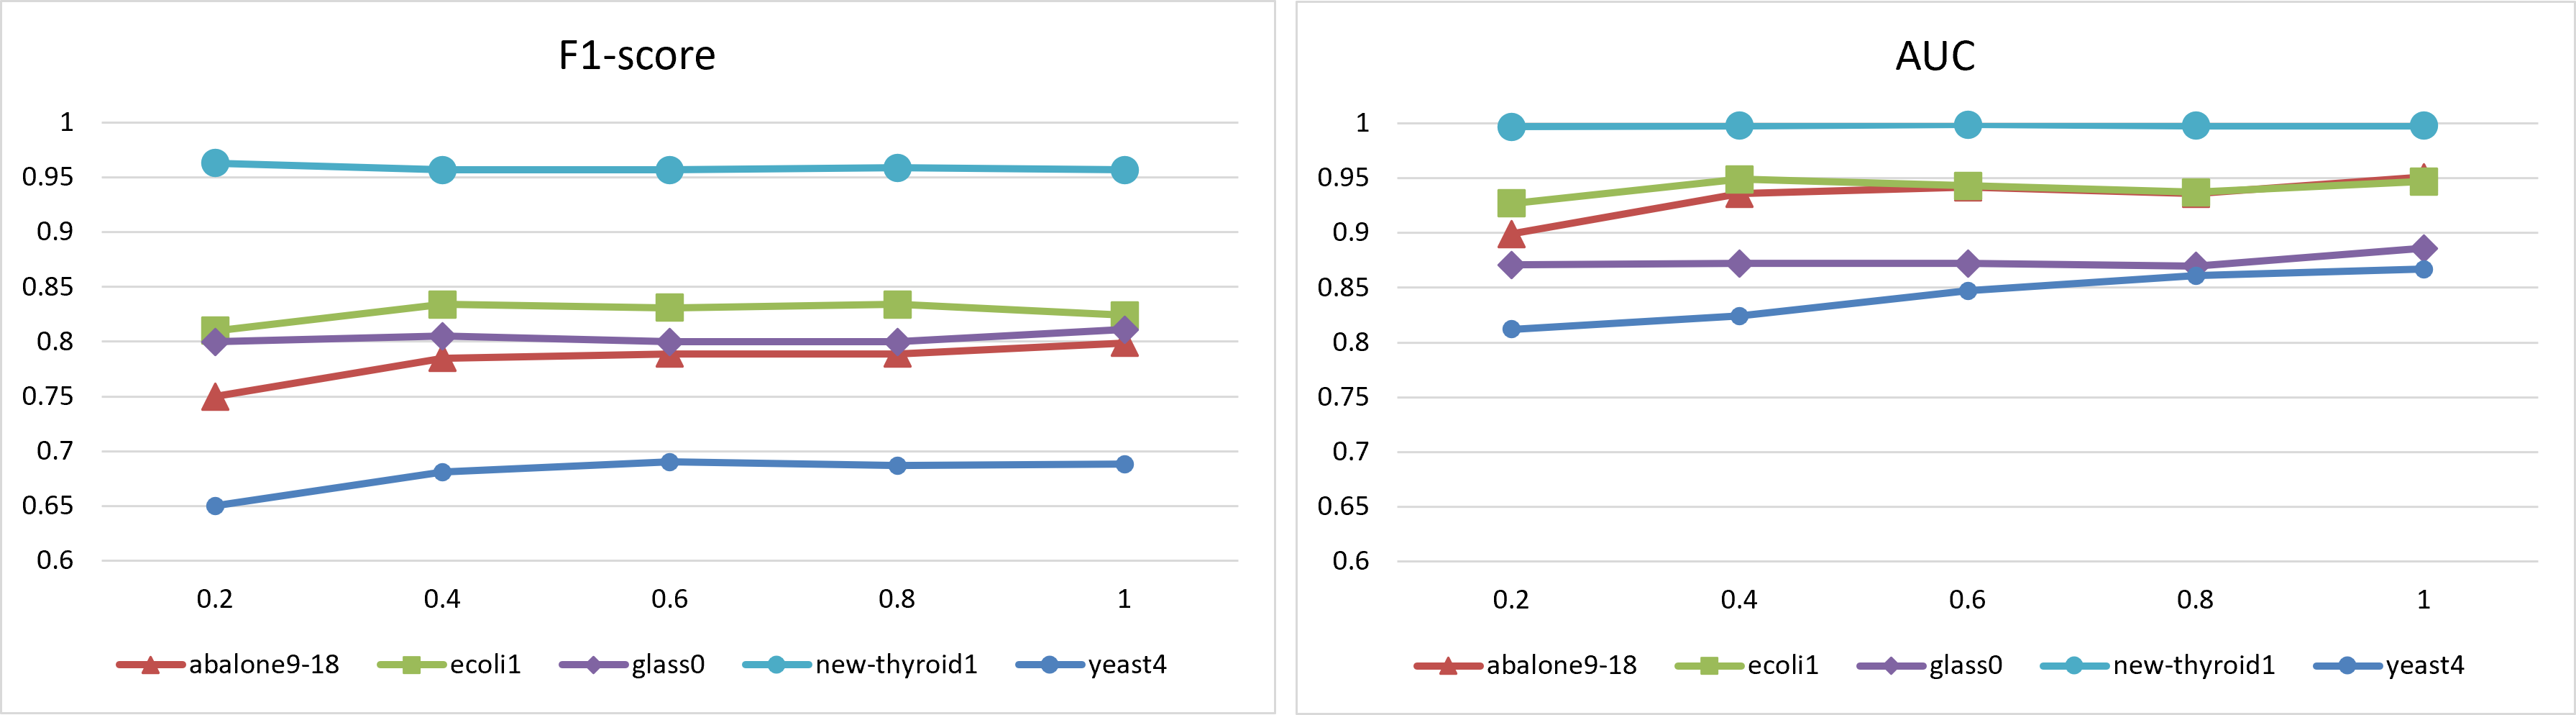
\includegraphics[width=0.98\linewidth, trim=5 10 10 10, clip ]{\ChapterPathSIMPOR/Figures/r_impact}
	\caption{F1-score and AUC results with varying Gaussian standard deviation.}
	\label{fig:r_result}
\end{figure*}


\subsection{Empirical Study on the Impact of Informative Portion}
This section studies the empirical impact of the informative portion (IP) in Section \ref{sec:EAL}. This portion works as a threshold to adjust how many samples are taken into consideration of informative samples. To save space, we study five datasets used in Section \ref{sec:simpor_r_distribution_impact}. Different values of IP ranging from 0.1 to 1 are applied, and the classification performance results are shown in Figure \ref{fig:ip_result}.

As we observe from the figure, while the performance is not significantly affected to datasets achieved high performance (new-thyroid1, ecoli1), there are obvious peaks within the IP values of (0.2, 0.6) in both F1-score and AUC score for other datasets (abalone9-18, glass0, yeast4). This suggests that tuning IP for each dataset between a range of (0.2, 0.6) could achieve higher performance. For example, by adjusting IP from 0.1 to 0.3 in ablalone9-18 dataset experiment, we can increase the performance by 5\% for both F1-score and AUC score. 

\begin{figure*}[h]
	\centering
	%[trim=left bottom right top, clip]
	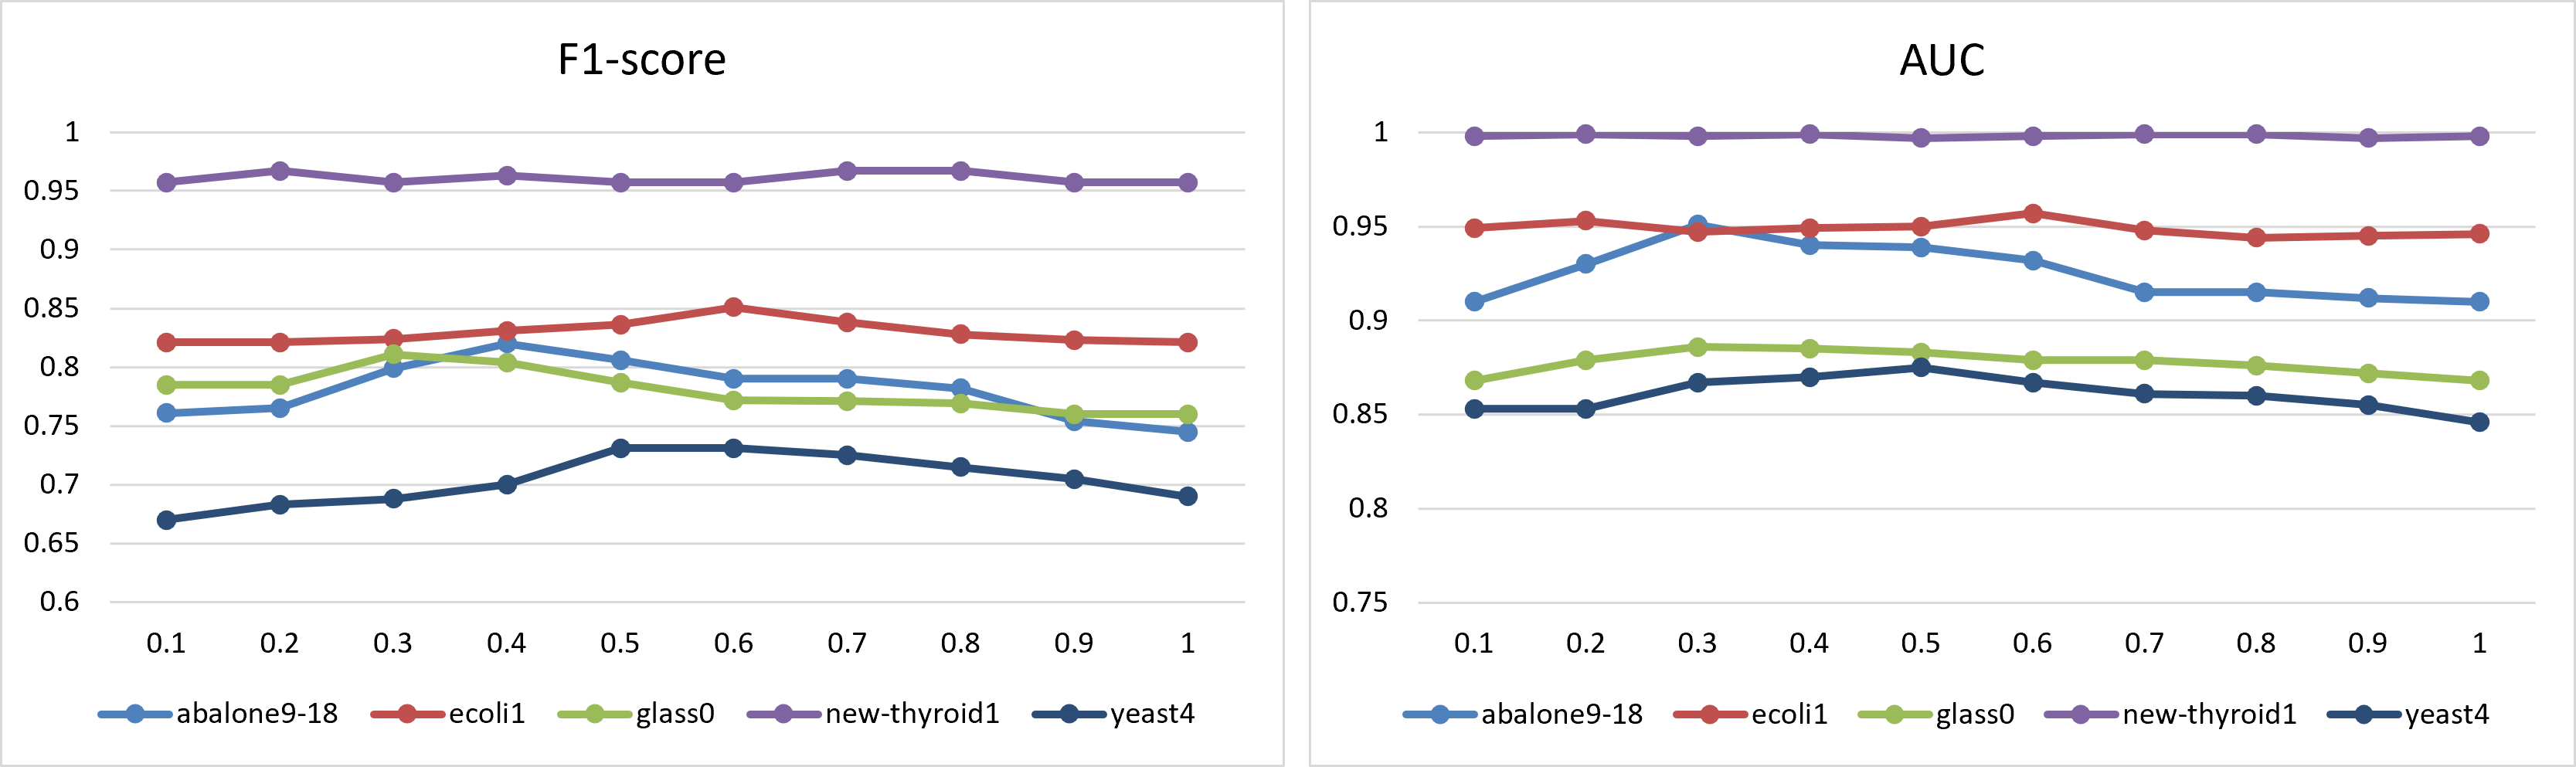
\includegraphics[width=0.98\linewidth, trim=5 10 10 10, clip ]{\ChapterPathSIMPOR/Figures/threshold_impact}
	\caption{F1-score and AUC results with varying informative portion IP.}
	\label{fig:ip_result}
\end{figure*}





